\documentclass[letterpaper,12pt,fleqn]{article}
\usepackage{matharticle}
\pagestyle{plain}
\begin{document}
\section*{Lab 6: Domains}

The domain for a function can be stated either explicitly or must be determined
implicitly. The latter can be a tricky proposition. In lecture, we discussed
three rules/guidelines for determining domains. We start by assuming all real
numbers and then throw out values that violate one of these three rules:
\begin{enumerate}
\item No zero denominators
\item No negative radicands in even radicals in numerator factors
\item No negative or zero radicands in even radicals in denominator factors
\end{enumerate}
Consider the following example:
\[f(x)=\frac{\sqrt{(x-1)(x+3)}}{(x-2)\sqrt[3]{x+1}}\]
We need to examine this problem bit by bit to see where rule violations can
occur. In the denominator, it is clear that $x\ne2$ because it would violate
rule 1. But do we need to worry about the $\sqrt[3]{x+1}$ factor? Since it is
an odd root we don't have to worry about rule 3, but we still need $x\ne-1$ so
as to not violate rule 1. As far as the numerator goes, we must solve the
inequality $(x-1)(x+3)\ge0$ so as to not violate rule 2. This yields
$(-\inf,-3]\cup[1,\infty)$.

So we have three criteria that we must meet:
\begin{enumerate}
\item $x\ne2$
\item $x\ne-1$
\item $x\in(-\inf,-3]\cup[1,\infty)$
\end{enumerate}
All three of these criteria must hold, so we actually want the intersection
of these three things. Note that the third criterion already excludes $x=-1$,
so we just need to make a hole at $x=2$:
\[x\in(-\inf,-3]\cup[1,2)\cup(2,\infty)\]

Another important rule for determining domains is that domains must be
determined based on how the function is initially presented to you. You must
keep in mind that simplifications may hide domain issues! Consider the
following example:
\[f(x)=\frac{\sqrt{(x-1)(x-2)}}{\sqrt{(x-1)(x-3)}}\]
It is very tempting to rewrite this as:
\[f(x)=\sqrt{\frac{(x-1)(x-2)}{(x-1)(x-3)}}\]
And then cancel the $x-1$ to get:
\[f(x)=\sqrt{\frac{x-2}{x-3}}\]
But this would be incorrect for domain purposes! Consider the value $x=1$.
This value looks perfectly fine for the reduced form, but would violate
rule 3 in the original form, so we make sure that we exclude it from the
domain. Likewise, $x=2$ is fine for the reduced form, but violates rule 3 in
the original form.

Instead, we must determine domain criteria for the numerator and denominator
separately and then take the intersection. Doing this yields the following:

\begin{tabular}{ll}
  numerator & $(-\infty,1]\cup[2,\infty)$ \\
  denominator & $(-\infty,1)\cup[3,\infty)$
\end{tabular}

Note that in the numerator the endpoints are included, but in the denominator
the endpoints are excluded (so as to not get a zero denominator). So we need
the intersection of these two criteria. The best way to find this is to plot
them on top of each other and use the endpoints to divide up the number line
into regions and then only include regions (and endpoints) that occur in
both criteria:

\vspace{0.25in}

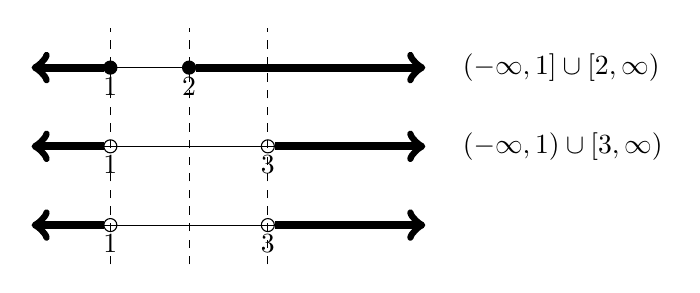
\begin{tikzpicture}
  \draw (0,2) -- (5,2) node [right] {$\quad(-\infty,1]\cup[2,\infty)$};
  \node [draw,circle,fill=black,scale=0.5] (a) at (1,2) {};
  \node [below] at (a) {$1$};
  \node [draw,circle,fill=black,scale=0.5] (b) at (2,2) {};
  \node [below] at (b) {$2$};
  \draw [<-,line width=1mm] (0,2) to (a);
  \draw [->,line width=1mm] (b) to (5,2);
  \draw (0,1) -- (5,1) node [right] {\quad$(-\infty,1)\cup[3,\infty)$};
  \node [draw,circle,scale=0.5] (c) at (1,1) {};
  \node [below] at (c) {$1$};
  \node [draw,circle,scale=0.5] (d) at (3,1) {};
  \node [below] at (d) {$3$};
  \draw [<-,line width=1mm] (0,1) to (c);
  \draw [->,line width=1mm] (d) to (5,1);
  \draw [dashed] (1,-0.5) -- (1,2.5);
  \draw [dashed] (2,-0.5) -- (2,2.5);
  \draw [dashed] (3,-0.5) -- (3,2.5);
  \draw (0,0) -- (5,0);
  \node [draw,circle,scale=0.5] (e) at (1,0) {};
  \node [below] at (e) {$1$};
  \node [draw,circle,scale=0.5] (f) at (3,0) {};
  \node [below] at (f) {$3$};
  \draw [<-,line width=1mm] (0,0) to (e);
  \draw [->,line width=1mm] (f) to (5,0);
\end{tikzpicture}

\vspace{0.25in}

So the final answer is that the domain of the original function is
\[(-\infty,1)\cup[3,\infty)\]
Note that this is the same as the denominator criterion, since the denominator
criterion is a subset of the numerator criterion.

Make sure you can follow all of the steps in the above problem!

\newpage

Now you try a problem. Consider the rather ugly function:
\[f(x)=\frac{(x^2-49)\sqrt[4]{x^2+3x+2}\sqrt{x^2-9}}
   {(x-7)\sqrt[5]{x^2-5x+6}\sqrt[6]{x^2-5x-6}}\]
Lot's of stuff going on here. The first step is to identify everything that
may be a problem. We do this factor by factor. Here are the six factors in
the problem. Write a number from $1$ to $3$ by each factor to indicate which of the
three rules might apply. If no rules apply then write ``none.'' Be sure to distinguish
between how the rules apply to even roots versus odd roots.
\begin{enumerate}
\item $x^2-49$
\item $\sqrt[4]{x^2+3x+2}$
\item $\sqrt{x^2-9}$
\item $x-7$
\item $\sqrt[5]{x^2-5x+6}$
\item $\sqrt[6]{x^2-5x-6}$
\end{enumerate}

The next step is to factor each of the individual factors. Make sure that you
get this correct or the whole problem goes haywire!
\begin{enumerate}
\item
\item
\item
\item
\item
\item
\end{enumerate}

Next, determine the criteria for each factor. Note that for even roots you
will need to solve a $\ge0$ inequality with the radicand. Your answers should be
either: ``none'', $x\ne a$ for some $a\in\R$, or something in interval notation.

\begin{enumerate}
\item
\item
\item
\item
\item
\item
\end{enumerate}

Three of the above answers should have been in interval notation. Graph them
one on top of each other. Make sure that the endpoint values are positioned
relative to one another. Then, use the endpoints to break up the number line
into regions and take the intersection. The final intersection should be a union
of two intervals. Be careful with inclusion/exclusion of endpoints.

\vspace{0.25in}

\begin{minipage}{\textwidth}
  \centering
  \begin{tikzpicture}
    \draw (-5,0) to (5,0);
    \draw (-5,1) to (5,1);
    \draw (-5,2) to (5,2);
    \draw (-5,3) to (5,3);
  \end{tikzpicture}
\end{minipage}

\vspace{0.25in}

Now review the other criteria to see if they introduce any holes. There is
indeed one. Where is there a hole in the above intersection?

\vspace{0.5in}

Graph the final answer for the domain of $f(x)$ and write the answer in
interval notation:

\vspace{0.25in}

\begin{minipage}{\textwidth}
  \centering
  \begin{tikzpicture}
    \draw (-5,0) to (5,0);
  \end{tikzpicture}
\end{minipage}

\vspace{0.25in}

$x\in$

\end{document}
